\documentclass[letterpaper]{article}
\usepackage{import}{\tiny }
\usepackage{standalone}
\usepackage[english]{babel}
\usepackage[a4paper]{geometry}
\usepackage[utf8]{inputenc}
\usepackage{float}
\usepackage{amsmath}
\usepackage{amssymb}
\usepackage{amsthm}
%\usepackage{cool} %seems cool. has bugs. conflicts with own derivative commands (below)
\usepackage{enumitem}
\usepackage{fancyhdr}
\usepackage{multirow}
\usepackage{booktabs}
\usepackage{subfiles}
\usepackage{siunitx}
\usepackage{graphicx}
\usepackage{caption}
\usepackage{subcaption}
\usepackage{hyperref}
\usepackage{appendix}
\usepackage{rotating}
\pagestyle{fancy}

%Packages and settings for code formatting
\usepackage{color}
\definecolor{code_keywords}   {rgb}{0,0,0} %blue={0.13,0.13,0.75}
\definecolor{code_comments}   {rgb}{0.17,0.57,0.17}
\definecolor{code_linenumbers}{rgb}{0.5,0.5,0.5}
\definecolor{code_strings}    {rgb}{0,0,0} %red={0.5,0,0}
\usepackage{listings}
\lstset{
	language		 = Matlab,
	basicstyle		 = \footnotesize,
	commentstyle	 = \color{code_comments},
	keywordstyle	 = \bfseries\color{code_keywords},
	stringstyle		 = \color{code_strings},
	numberstyle		 = \tiny\color{code_linenumbers},
	frame			 = none,
	keepspaces		 = true,
	numbers			 = left,
	numbersep		 = 5pt,
	showspaces		 = false,
	showstringspaces = false,
	showtabs		 = false,
	stepnumber		 = 1,
	tabsize			 = 4,
}


\lfoot{} % Controls the left corner of the footer
\cfoot{} % Controls the center of the footer
\rfoot{page~\thepage} % Controls the right corner of the footer
\renewcommand{\headrulewidth}{0.4pt}
\renewcommand{\footrulewidth}{0.4pt}

%Specify table columns' width
\newcolumntype{L}[1]{>{\raggedright\arraybackslash}p{#1}}
\newcolumntype{C}[1]{>{\centering\arraybackslash}p{#1}}
\newcolumntype{R}[1]{>{\raggedleft\arraybackslash}p{#1}}


\newcommand{\todo}[1]{\textcolor{red}{\textbf{[TODO]}~#1}}

\newcommand{\imp}{\Rightarrow} %mathematical "implies"
\newcommand{\Imp}{\quad\imp\quad} %...with spacing


\author{Giovanni Bologni (4757386) and Wouther Bons (4092716)}
\date{\today}
\title{EE4389\\Modeling and Data Analysis in Complex Networks\\Assignment}
\lhead{EE4389 Complex Networks Assignment} % Controls the left corner of the header
\chead{} % Controls the center of the header
%\rhead{Giovanni Bologni and Wouther Bons} % Controls the right corner of the header

\begin{document}
\maketitle

\subsection*{Introduction}
When measurements are performed on a network, the resulting dataset can be analysed to quantify properties of the underlying network. In this assignment a dataset of face-to-face contact data of highschool students\footnote{R. Mastrandrea, J. Fournet, A. Barrat, Contact patterns in a high school: a comparison between data collected using wearable sensors, contact diaries and friendship surveys. PLoS ONE 10(9): e0136497 (2015)} is analysed.

This data not only includes contact information at a certain time, but also how contact changes over time; every measurement specifies which two students have had contact and at which time this occured. Students will be modeled as nodes in a graph and contact between students as edges. Each edge will also be labeled with the timestamp at which the contact it represents was made.

To begin with, this data will be aggregated over all time to analyse the topology of the resulting aggregated network. Secondly, the time of measurement will be taken into consideration. Several metrics will be used to analyse which nodes are most influential when information spreads across this temporal network. Lastly, temporal features of the network will be altered to inspect their influence on the information spreading process.

\subsection*{Part A: Topological features of the aggregated network}
\label{sec:partA}

All measured topological features are summarized in table \ref{tab:topological_features}.

%\setlength\LTleft{0pt} % left-align rather than center-set the longtable
\begin{table}[!ht]
	\centering
	\begin{tabular}{@{} L{10em} L{5em} R{2.5em} @{} L{2.5em} @{}}
	\toprule
	\textbf{Topological feature} & ~ & \multicolumn{2}{r}{\textbf{Value}}\\
	\midrule
	Number of nodes& N & 327& \\
	Number of links& L & 5818& \\ 
	Link density& p  & 0&.1092 \\ 
	Average degree& $E[D]$  & 35&.58\\
	Degree variance& $Var[D]$ & 182&.2 \\
	Degree assortativity& $\rho_D$ & 0&.03318\\
	Clustering coefficient& C & 0&.5035\\
	Average hopcount& $E[H]$ & 2&.159\\
	Diameter& $H_{max}$ & 4& \\
	Spectral radius& $\lambda_1$ & 41&.23\\
	Algebraic connectivity& $\mu_{N-1}$ & 1&.93\\
	\bottomrule
	\end{tabular}
	\caption{List of all topological features of the aggregated network that were examined. For details on calculations and interpretations see part \ref{sec:partA}.}
	\label{tab:topological_features}
\end{table}

The aggregated graph \(G\) is constructed by connecting any two nodes by an (unweighted) edge if the nodes make contact with eachother at least once in the \(T=7375\) timesteps available.


The link density is computed as
\begin{align*}
p = \frac{L}{L_{max}} = \frac{L}{N(N-1)/2} = 0.1092
\end{align*}

Several metrics inspect the degree of nodes in the network, of which an insightful one is the degree distribution. From fig.~\ref{fig:degree_distribution_linlin}, it can be seen that this distribution resembles a Poisson distribution. This suggests that an Erdös-Renyi (ER) graph model would be well suited to model the face-to-face contact network. In contrast, a scale-free graph model would be a bad choice of model because scale-free graphs show a linear distribution when viewed on a log-log scale and this is absolutely not the case (fig.~\ref{fig:degree_distribution_loglog}).

The degree assortativity (\(\rho_D=0.03318\)) is defined as the (linear) correlation coefficient between the degrees of nodes. A high degree assortativity indicates that two nodes are more likely to be connected if their degrees are similar, while a value of almost zero, as in our case, means the degrees of nodes are not correlated at all.  
This means that the creation of new links in the aggregated graph is not influenced by existing links; another argument for using the ER graph model, where edges are created with independent probabilities (and are therefore uncorrelated).

\begin{figure}
    \centering
    \begin{subfigure}[b]{0.49\textwidth}
        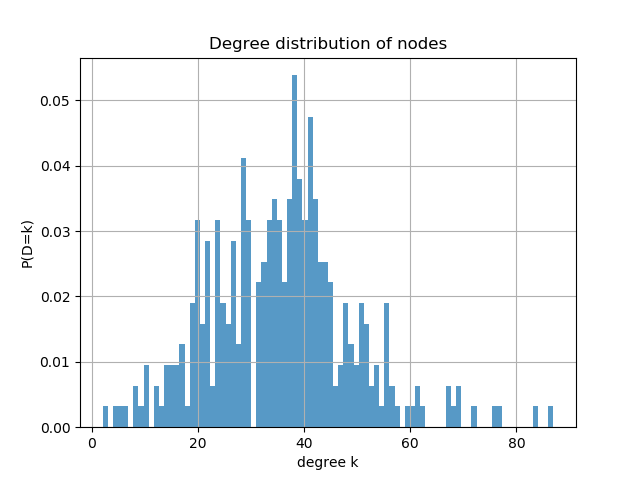
\includegraphics[width=\textwidth]{img/degree_distribution.png}
        \caption{Linear scale}
	    \label{fig:degree_distribution_linlin}
    \end{subfigure}
    ~ % spacing
    \begin{subfigure}[b]{0.48\textwidth}
        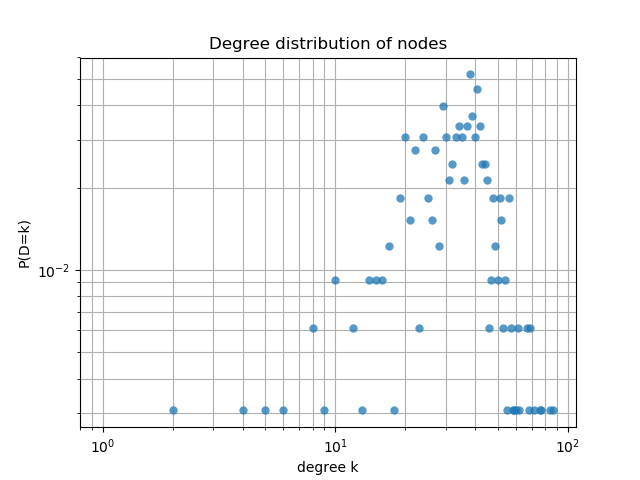
\includegraphics[width=\textwidth]{img/degree_distribution_loglog.png}
        \caption{Log scale}
	    \label{fig:degree_distribution_loglog}
    \end{subfigure}
    \caption{Degree distribution of nodes in the aggregated graph.}
    \label{fig:degree_distribution_aggregated}
\end{figure}

Furthermore, it is interesting to check whether the network exhibits the small-world property, i.e. if it the nodes are strongly clustered and the average distance among them is only a few hops. 
Comparing the clustering coefficient (\(C=0.5035\)) and average hopcount (\(E[H]=2.159\)) to the same metrics evaluated on a regular graph (with a similar average degree) results in the following ratios: 

\begin{align*}
C/C(0) = 4.681\\
E[H]/E[H](0) = 1.132
\end{align*}

Because the clustering coefficient on the aggregated graph is more than 4 times higher then in the regular graph, while the average hopcounts are comparable in the two graphs, the network exhibits the small-world property. 

Comparing the average hopcount (\(E[H]=2.159\)) with the diameter of the graph (\(H_{max}=4\)) we see that there is not a lot of variance in hopcounts of shortest paths between nodes; the diameter (the worst-case hopcount of shortest paths) is close to the graph's efficiency (the average hopcount). This again points to the small-world property.

Lastly, some spectral metrics of the aggregated graph are considered. The spectral radius is calculated as the largest eigenvalue of the adjacency matrix \(\lambda_1=41.23\). The algebraic connectivity is the second smallest eigenvalue of not the adjacency but the Laplacian matrix, \(\mu_{N-1}=1.930 > 1\). This ensures that the graph is connected; as a consequence, we shall see in Part B that all the nodes from the graph contract the infection, no matter what node will be chosen to start the infection propagation.


\subsection*{Part B: Information spreading on a temporal network}

As mentioned in the introduction, each edge was labeled with the timestamp at which the contact between students it represents was made. This means we can simulate the spread of information over the time network \(G_{data}\) over time. 
The information spreading process used is as follows: an infected node can infect any nodes it is in contact with (i.e. its neighbours at a specific timestamp), but these neighbours can only start infecting other nodes at the next timestamp. Infection starts with some selected seed node. 
This simulation is done N times; every node is a seed node once. Graphs of the number of infected nodes \(I(t)\) (fig.~\ref{fig:infections_G}) shows the average \(E[I(t)]\) as well as the standard deviation \(\sqrt{Var[I(t)]}\) over these N simulations.
\begin{figure}[ht!]
  \centering
   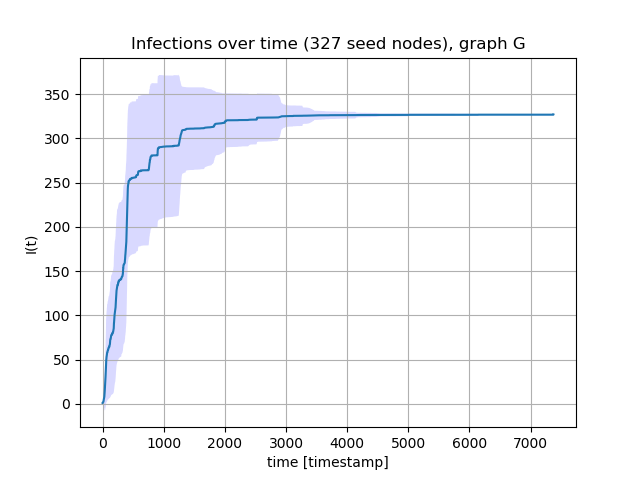
\includegraphics[width=0.65\textwidth]{img/infections_G.png}
   \caption{\small{The average number of infected nodes as a function of the time step, $\mathrm{E}[I(t)]$, on the temporal graph $G_{data}$. The standard deviation, $\sqrt{\mathrm{Var}{[I(t)}]}$ is indicated by the shaded area.}}
   \label{fig:infections_G}
\end{figure}

One metric used to quantify how fast information spreads over the temporal network is the timestamp at which 80\% of all nodes have been infected. For every simulation the seed node and timestamp of 80\% infection is recorded. By sorting the seed nodes by their 80\% infection timestamps, the nodes are ranked according to their influence as a seed node, i.e. \(R=[R_{(1)}, R_{(2)}, ..., R_{(N)}]\). This ordering can now be used as a standard to quantify nodes' influence. Using the same process nodes can be ranked using other metrics (e.g. the degree, \(D=[D_{(1)}, D_{(2)}, ..., D_{(N)}]\)) and subsequently compared with R by checking how many nodes are in the same top-f fraction for both metrics, R and D. This is called the top-f recognition rate and is calculated as:
\begin{align*}
	r_{RD}(f) = \frac{\left|R_f \cap D_f\right|}{\left|R_f\right|},
\end{align*}

\noindent Several metrics are compared to R using this procedure. The results can be found in figure \ref{fig:rankG}. The temporal metrics were calculated as follows at each timestamp \(t\), for each node \(i\):

\begin{align*}
	TD_i &= \frac{D_i}{t^2+t},\\
	XTD_i &= 
		\begin{cases}
		\frac{D_i}{t}& \text{if node connected to new neighbours at this timestamp,}\\
		0& otherwise,
		\end{cases}
\end{align*}
\noindent where \(D_i\) is the degree of the \(i\)-th node.

The reasoning behind these metrics is that earlier contacts are more influential than later ones. For example, at later timestamps a significant part of contacts happen between infected nodes, thus not contributing to the infection spread. The temporal degree (TD) tries to account for this reduced nodal influence at later timestamps by weighting the degree with something inversely propertional to the timestamp. 
Additionally, the exclusive temporal degree (XTD) discards (i.e. zero weight) any repeated contact between nodes.

Figure \ref{fig:rankG} shows the results of these temporal metrics on the graph \(G_{data}\), as well as several non-temporal ones, evaluated on \(G\). 

\begin{figure}[ht]
  \centering
   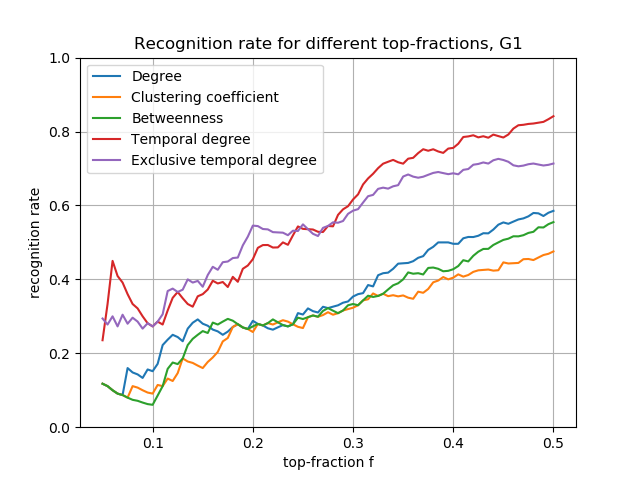
\includegraphics[width=0.7\textwidth]{img/rankG.png}
   \caption{\small{The top $f$ recognition rate $r_{RX}(f) = \frac{ |R_f \cap X_f| }{ |R_f| }$, where $R_f$ and $X_f$ are the sets of nodes ranking in the top $f$ fraction according to their influence,  or to another metric $X(f)$, respectively. The metrics based on the temporal features, TD and XTD, are more accurate in detecting the most influential seed nodes.}}
   \label{fig:rankG}
\end{figure}

Because the comparison is done as a fraction the ideal metric would yield a unity recognition rate, i.e. ranking nodes' influence using that metric yields exactly the same results as ranking by 80\% infection timestamps (R). 
On the other side, a linear recognition rate with unit slope means that using the metric to rank nodal influence performs the same as tossing a coin, e.g. if 40\% of nodes in the top-40\% match with R.
%Therefore a value closer to unity in figure~\ref{fig:rankG} means a better metric. 

With this in mind, it is clear that both temporal metrics perform better than non-temporal ones, which is to be expected as they use more information.
It should be noted, however, that neither the degree, clustering coefficient nor betweenness of the aggregated graph are significantly better than random chance at predicting nodal influence.

% question 13:
%\todo{not really sure about this... even though it's beautifully written, it's really long and not strictly necessary, since we're considering only big networks. Maybe you can find a way to cut it?}
One caveat of using the top-f recognition rate is that it artifically separates nodes for which a metric has the same value. For example, consider a small graph of five nodes, where node 1 through 4 all have degree 1 and node 5 has a higher degree. The ranking nodes by degree could then be any permutation of nodes 1 through 4, followed by 5, e.g. \(D=[D_{(1)},D_{(2)},D_{(3)},D_{(4)},D_{(5)}]\) or \(D=[D_{(2)},D_{(4)},D_{(1)},D_{(3)},D_{(5)}]\). The top-f recognition rate then depend on the permutation of nodes with equal degree, while in reality the nodes perform equally well and should theoretically all four "share" first place. This effect is neglegible for very large networks but is important to take into consideration when using top-f recognition rates for smaller networks.


\subsection*{Part C: Influence of temporal network features on information spreading}
\label{sec:partC}

In Part A, several topological features of the aggregated graph \(G\) were evaluated. 
It was shown how \(G\) has the typical connectivity properties of a Watts-Strogatz graph, while the degree distribution resembles a Poisson distribution, as in the ER graph. 
In Part B, we simulated an infection process and ranked the nodes according to the propagation rate. Moreover, several temporal and non-temporal metrics were proposed to predict the influence of the seed nodes.

\noindent Let us now consider the information spreading process on two randomized graphs:
\begin{itemize}
\item \(G_2\), which has the same temporal links as \(G_{data}\), while the time stamps are reshuffled,
\item \(G_3\), that is obtained by randomizing and re-aggregating the original graph \(G\).
%  with the timestamps randomly redistributed across the edges.
\end{itemize}

\noindent The average numbers of infected nodes per time stamp on the graphs \(G_{data}\), \(G_2\) and \(G_3\) are plotted in fig.~\ref{fig:infections_over_time}. 

\noindent The infection spread in the shuffled graph, \(G_2\), is significantly faster than in the original graph. A likely explanation is that the rewiring process, while leaving the degrees on the aggregated graph untouched, changes drastically the order in which the links are formed. Therefore, the typical causality of the real-world data is lost: whereas two connected nodes in \(G_{data}(t)\) were very likely to be connected in \(G_{data}(t+1)\), the edges in \(G_2(t)\) are completely independent from the edges in \(G_2(t+1)\), thus contributing to the infection spread.
These interpretations are quantitatively supported by fig.~\ref{fig:degree_distribution}, which shows the amount of new nodes appearing in the temporal graphs at the beginning of the infection spread. 

Similarly, all the nodes in \(G_3\) get infected after a relatively short time, with low variance.
\(G_3\) is constructed by first taking a copy of the aggregated graph \(G\), where all the edges only appear once, then randomizing the edges and then aggregating the resulting graph. This way, some edges disappear together with the linked nodes, since they are not assigned any time stamp.

The metrics proposed in Part B do not reliably predict the most influential seed nodes in \(G_2\) and \(G_3\) (fig.~\ref{fig:recognition_rates}. An alternative performance measure could take into account the number of new neighbours of a node in a time window. As an example, the activity potential of a node is defined as the number of interactions that the node had in a given time window, divided by the total number of interactions made by all nodes during the same time slot.
On the other hand, when we are interested in the global behaviour of a graph, recent studies suggest that spectral metrics seem to be essential in network characterizations. 

\begin{figure}
    \centering
    \begin{subfigure}[b]{0.32\textwidth}
        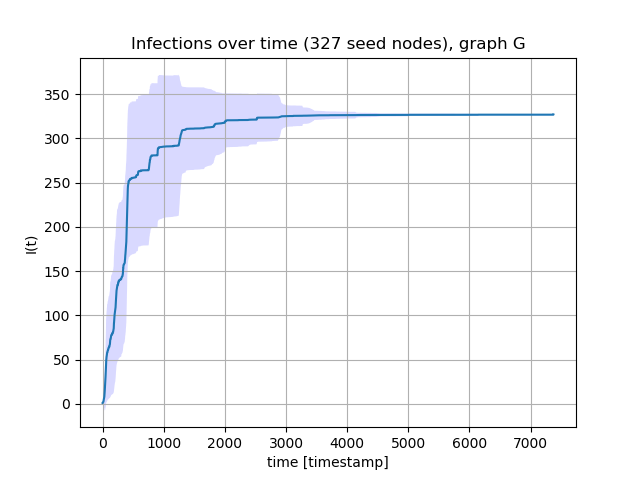
\includegraphics[width=\textwidth]{img/infections_G.png}
        \caption{Graph \(G_{data}\)}
	    \label{fig:infections_over_time_G}
    \end{subfigure}
%    ~ % spacing
    \begin{subfigure}[b]{0.32\textwidth}
        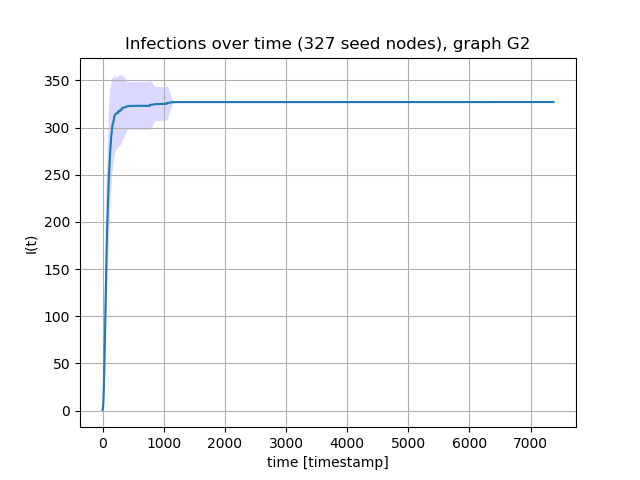
\includegraphics[width=\textwidth]{img/infections_G2.png}
        \caption{Graph \(G_2\)}
	    \label{fig:infections_over_time_G2}
    \end{subfigure}
%     ~ % spacing
    \begin{subfigure}[b]{0.32\textwidth}
        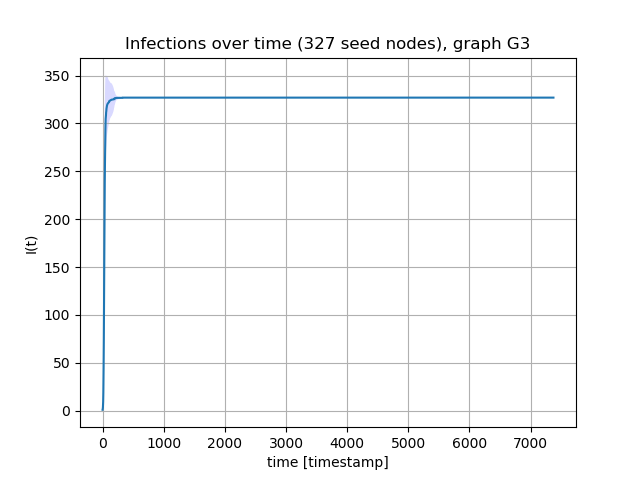
\includegraphics[width=\textwidth]{img/infections_G3.png}
        \caption{Graph \(G_3\)}
	    \label{fig:infections_over_time_G3}
    \end{subfigure}
    \caption{\small{The average number of infected nodes as a function of the time step, $\mathrm{E}[I(t)]$ on several temporal graphs. The standard deviation, $\sqrt{\mathrm{Var}{[I(t)}]}$ is indicated by the shaded area. The propagation speed increases when the original graph is reshuffled.}}
    \label{fig:infections_over_time}
	
	\bigskip
	
    \centering
    \begin{subfigure}[b]{0.32\textwidth}
        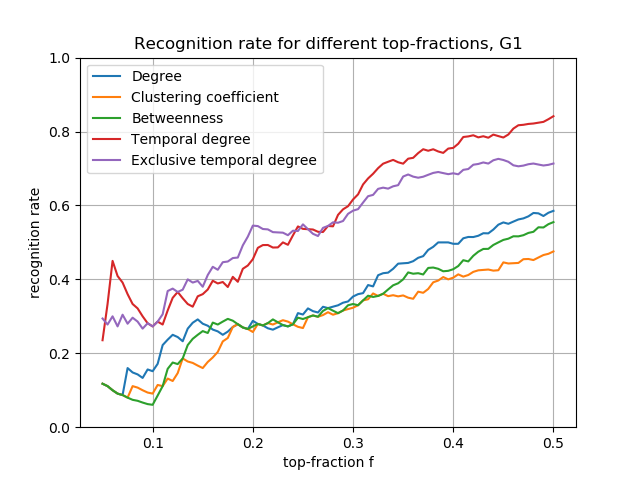
\includegraphics[width=\textwidth]{img/rankG.png}
        \caption{Graph \(G_{data}\)}
	    \label{fig:recognition_rates_G}
    \end{subfigure}
%    ~ % spacing
    \begin{subfigure}[b]{0.32\textwidth}
        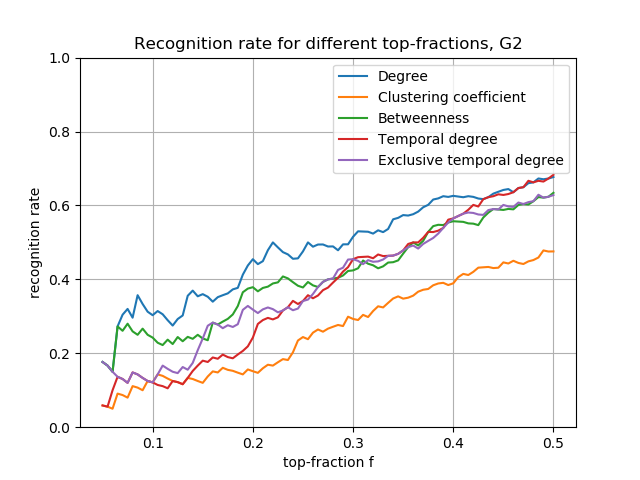
\includegraphics[width=\textwidth]{img/rankG2.png}
        \caption{Graph \(G_2\)}
	    \label{fig:recognition_rates_G2}
    \end{subfigure}
%     ~ % spacing
    \begin{subfigure}[b]{0.32\textwidth}
        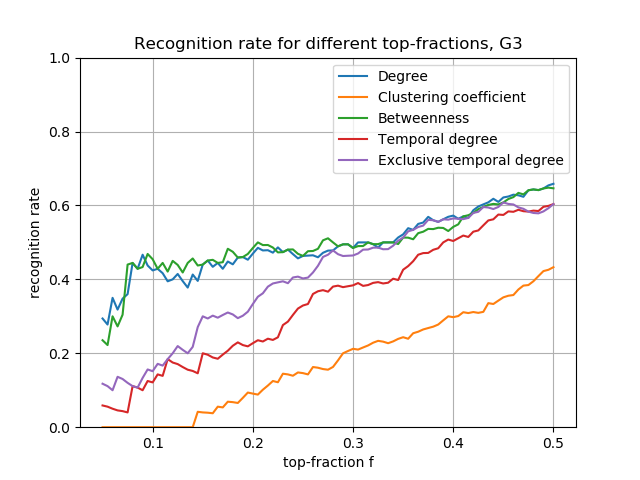
\includegraphics[width=\textwidth]{img/rankG3.png}
        \caption{Graph \(G_3\)}
	    \label{fig:recognition_rates_G3}
    \end{subfigure}
    \caption{\small{The top $f$ recognition rate $r_{RX}(f) = \frac{ |R_f \cap X_f| }{ |R_f| }$ for different metrics, evaluated on the three temporal graphs. All the proposed metrics seem inappropriate to detect the most influential spreaders on the randomized graphs, being just above chance performance.}}
    \label{fig:recognition_rates}
	
	\bigskip
	
    \centering
    \begin{subfigure}[b]{0.32\textwidth}
        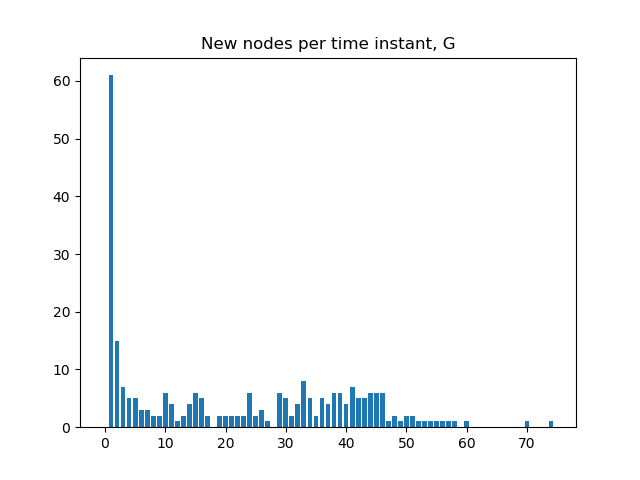
\includegraphics[width=\textwidth]{img/newNodesG.png}
        \caption{Graph \(G_{data}\)}
	    \label{fig:degree_distribution_G}
    \end{subfigure}
%    ~ % spacing
    \begin{subfigure}[b]{0.32\textwidth}
        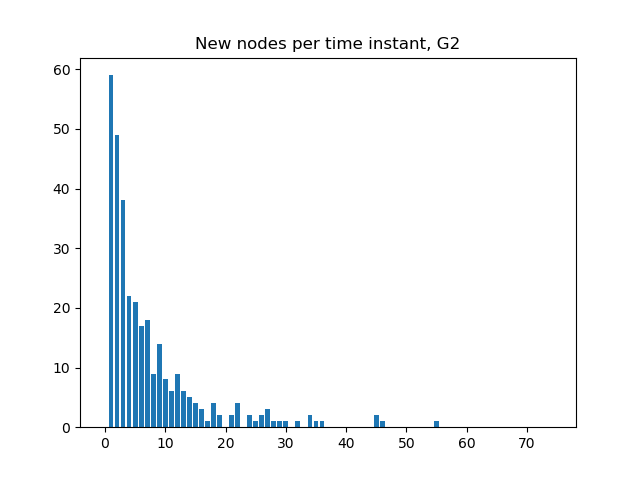
\includegraphics[width=\textwidth]{img/newNodesG2.png}
        \caption{Graph \(G_2\)}
	    \label{fig:degree_distribution_G2}
    \end{subfigure}
%     ~ % spacing
    \begin{subfigure}[b]{0.32\textwidth}
        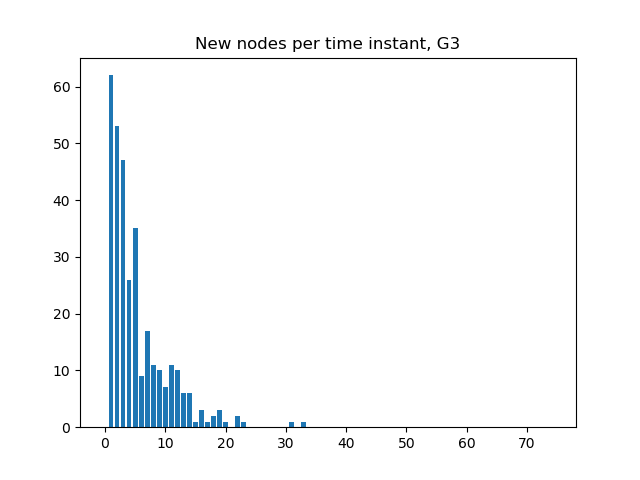
\includegraphics[width=\textwidth]{img/newNodesG3.png}
        \caption{Graph \(G_3\)}
	    \label{fig:degree_distribution_G3}
    \end{subfigure}
    \caption{\small{Number of new nodes added to the graph at timestamp \(t\). 
    The plots focuse on the initial phase of the spreading process: the x-axis ranges from 0 to \(T=100\). It is apparent how the two randomized graphs, \(G_2\) and \(G_3\), get connected to a larger number of previously unseen nodes, thus contributing to the infection spread. }}
    \label{fig:degree_distribution}
\end{figure}

\end{document}
